\documentclass[11pt,a4paper]{article}
\usepackage[a4paper,top=14mm,bottom=14mm,left=15mm,right=15mm]{geometry}
\usepackage[T1]{fontenc}
\usepackage{amsmath}
\usepackage{amssymb}
\usepackage{array}
\usepackage{multicol}
\usepackage{tikz}
\usetikzlibrary{arrows.meta}

% ================================================================
% Standard form: revision questions.
%
% Two pages of questions, in black and white, with a heading for each
% topic on the Maths Revision topic list in the same order. Each topic
% has a few short questions that start easy, with a diagram only where
% a question uses one, and the sheet ends with some problem solving.
% There are no key facts or worked examples on the sheet: the methods
% are in the worked solutions and the revision guide. Questions are
% numbered through the sheet so that the answer key and the worked
% solutions can refer to them.
% ================================================================

\pagestyle{empty}
\setlength{\parindent}{0pt}
\setlength{\parskip}{2pt}
\setlength{\columnsep}{9mm}

% A topic from the revision list.
\newcommand{\topic}[1]{\par\addvspace{9pt}{\bfseries #1}\par\nobreak\vspace{2pt}}

% Questions are numbered through the whole sheet.
\newcounter{qn}
\newcommand{\q}{\par\addvspace{5pt}\stepcounter{qn}\hangindent=1.6em\hangafter=1\noindent
  \makebox[1.6em][l]{\textbf{\theqn}}}

% A calculator key, drawn as a small box.
\newcommand{\calckey}[1]{{\setlength{\fboxsep}{1.5pt}\fbox{\small #1}}}

\begin{document}
% Ragged right, without \raggedright, which would make \\ end the
% paragraph and lose the hanging indent of a question's later lines.
\setlength{\rightskip}{0pt plus 4em}

{\Large\bfseries Standard form}\hfill{\large Revision questions}
\par\vspace{2pt}\hrule\vspace{4pt}

\begin{multicols}{2}

% ----------------------------------------------------------------
\topic{Writing large and small numbers in standard form}
\q The place value table shows the number 72\,500. Write 72\,500 in standard form.\\[4pt]
{\renewcommand{\arraystretch}{1.5}%
\begin{tabular}{|c|c|c|c|c|}\hline
$10^4$ & $10^3$ & $10^2$ & $10^1$ & $10^0$\\\hline
7 & 2 & 5 & 0 & 0\\\hline
\end{tabular}}
\q Write in standard form.\\
(a) 6000\qquad (b) 3\,080\,000\\
(c) 0.009\qquad (d) 0.000\,304
\q Write as ordinary numbers.\\
(a) $3\times10^6$\qquad (b) $2.07\times10^4$\\
(c) $5\times10^{-2}$\qquad (d) $6.1\times10^{-5}$
\q Two of these numbers are not written in standard form. Find them, and write them correctly.
\[ 34\times10^5\qquad 7\times10^{-2}\qquad 0.7\times10^3\qquad 1.5\times10^9 \]
\q The planet Mercury is about 58\,000\,000\,km from the Sun. Write this distance in standard form.
\q The table shows the widths of some small things. Write them in order, smallest first.\\[4pt]
{\renewcommand{\arraystretch}{1.5}%
\begin{tabular}{|l|c|}\hline
Grain of sand & $5\times10^{-4}$ m\\\hline
Human hair & $7\times10^{-5}$ m\\\hline
Red blood cell & $8\times10^{-6}$ m\\\hline
Ant & $4\times10^{-3}$ m\\\hline
\end{tabular}}

% ----------------------------------------------------------------
\topic{Multiplying and dividing in standard form}
\q Work out, giving your answers in standard form.\\[2pt]
(a) $(2\times10^3)\times(4\times10^5)$\\[2pt]
(b) $(5\times10^6)\times(3\times10^{-2})$\\[2pt]
(c) $(9\times10^8)\div(3\times10^2)$\\[2pt]
(d) $(2\times10^{-3})\div(8\times10^4)$
\q A sheet of paper is $1\times10^{-4}$\,m thick. How tall is a pile of $5\times10^3$ sheets? Give your answer in standard form.
\q Light travels $3\times10^5$\,km in one second. How far does light travel in $2\times10^3$ seconds?

% ----------------------------------------------------------------
\topic{Adding and subtracting in standard form}
\q Work out, giving your answers in standard form.\\[2pt]
(a) $6\times10^4+3\times10^3$\\[2pt]
(b) $8.5\times10^6-4\times10^5$\\[2pt]
(c) $2\times10^{-3}+6\times10^{-4}$\\[2pt]
(d) $7\times10^{-2}-5\times10^{-3}$
\q Ben says, ``$3\times10^4+2\times10^3=5\times10^7$.'' Explain Ben's mistake, and find the correct answer.
\q The diameter of Jupiter is $1.43\times10^5$\,km. The diameter of the Earth is $1.27\times10^4$\,km. How much bigger is the diameter of Jupiter? Give your answer in standard form.

\end{multicols}

\newpage

\begin{multicols}{2}

% ----------------------------------------------------------------
\topic{Standard form with a calculator}
\q Use a calculator. Give your answers in standard form.\\[2pt]
(a) $(6.3\times10^7)\times(4.8\times10^{-3})$\\[2pt]
(b) $(7.5\times10^4)^2$\\[2pt]
(c) $(9.6\times10^5)\div(1.2\times10^{-3})$\\[2pt]
(d) $\sqrt{4.9\times10^7}$\\[4pt]
On most calculators, standard form is entered with the \calckey{$\times10^x$} key.
\q Ava wants to work out $(4\times10^3)\div(2\times10^2)$. She types\\[3pt]
\calckey{4} \calckey{$\times$} \calckey{1} \calckey{0} \calckey{$x^\square$} \calckey{3} \calckey{$\div$} \calckey{2} \calckey{$\times$} \calckey{1} \calckey{0} \calckey{$x^\square$} \calckey{2} \calckey{$=$}\\[3pt]
and gets 200\,000. The correct answer is 20. Explain what has gone wrong.

% ----------------------------------------------------------------
\topic{Problems with standard form}
\q The Moon is $3.84\times10^8$\,m from the Earth. Light travels at $3\times10^8$\,m per second. How many seconds does light from the Moon take to reach the Earth?\\[4pt]
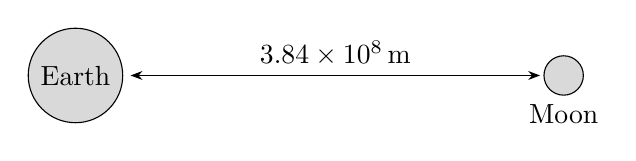
\begin{tikzpicture}[x=1mm,y=1mm]
  \draw[fill=black!15] (0,0) circle (6);
  \node at (0,0) {Earth};
  \draw[fill=black!15] (62,0) circle (2.5);
  \node[below=2.5mm] at (62,0) {Moon};
  \draw[{Stealth[length=1.5mm]}-{Stealth[length=1.5mm]}] (7,0) -- (59,0);
  \node[above] at (33,0) {$3.84\times10^8$\,m};
\end{tikzpicture}

\columnbreak
\q A spacecraft travels at $1.1\times10^4$\,m per second for one hour, which is $3.6\times10^3$ seconds. How far does it travel? Give your answer in standard form.
\q A red blood cell is $8\times10^{-6}$\,m wide. How many red blood cells would fit side by side across a fingernail $2\times10^{-2}$\,m wide?
\q The population of the UK is about $6.8\times10^7$. The area of the UK is about $2.4\times10^5$\,km$^2$. On average, how many people are there for each km$^2$? Give your answer to 2 significant figures.
\q The mass of the Earth is $5.97\times10^{24}$\,kg. The mass of the Moon is $7.35\times10^{22}$\,kg. How many times heavier is the Earth than the Moon? Give your answer to the nearest whole number.

% ----------------------------------------------------------------
\topic{Problem solving}
\q A computer does $3\times10^9$ calculations each second. How many hours does it take to do $1.2\times10^{14}$ calculations? Give your answer to 1 decimal place.
\q Two numbers in standard form are multiplied, and the answer is $6\times10^5$. Write down three different pairs of numbers that could have been multiplied.
\q Which is bigger, $(2\times10^3)^3$ or $10^{10}$? Show how you know.

\end{multicols}

\end{document}
